%%%%%%%%%%%%%%%%%%%%%%%%%%%%%%%%%%%%%%%%%%%%%%%%%%%%%%%%%%%%%%%%%%%%%%%%%%%%%%%%
%%%%%%%%%%%%%%%%%%%%%%%%%%%%%%%%%%%%%%%%%%%%%%%%%%%%%%%%%%%%%%%%%%%%%%%%%%%%%%%%
%%%%%%%%%%%%%%%%%%%%%%%%%%%%%%%%%%%%%%%%%%%%%%%%%%%%%%%%%%%%%%%%%%%%%%%%%%%%%%%%
%%%%%%%%%%%%%%%%%%%%%%%%%%%%%%%%%%%%%%%%%%%%%%%%%%%%%%%%%%%%%%%%%%%%%%%%%%%%%%%%
\chapter{Initiation à MATLAB\label{annexe-matlab}}
%%%%%%%%%%%%%%%%%%%%%%%%%%%%%%%%%%%%%%%%%%%%%%%%%%%%%%%%%%%%%%%%%%%%%%%%%%%%%%%%
%%%%%%%%%%%%%%%%%%%%%%%%%%%%%%%%%%%%%%%%%%%%%%%%%%%%%%%%%%%%%%%%%%%%%%%%%%%%%%%%
%%%%%%%%%%%%%%%%%%%%%%%%%%%%%%%%%%%%%%%%%%%%%%%%%%%%%%%%%%%%%%%%%%%%%%%%%%%%%%%%
%%%%%%%%%%%%%%%%%%%%%%%%%%%%%%%%%%%%%%%%%%%%%%%%%%%%%%%%%%%%%%%%%%%%%%%%%%%%%%%%
\input{re/newgeometry}
\captionsetup{width=0.9\linewidth}
%%%%%%%%%%%%%%%%%%%%%%%%%%%%%%%%%%%%%%%%%%%%%%%%%%%%%%%%%%%%%%%%%%%%%%%%%%%%%%%%
%%%%%%%%%%%%%%%%%%%%%%%%%%%%%%%%%%%%%%%%%%%%%%%%%%%%%%%%%%%%%%%%%%%%%%%%%%%%%%%%
%%%%%%%%%%%%%%%%%%%%%%%%%%%%%%%%%%%%%%%%%%%%%%%%%%%%%%%%%%%%%%%%%%%%%%%%%%%%%%%%
\section[Présentation générale]
        {Présentation générale 
        (\href{https://fr.wikipedia.org/wiki/MATLAB}{Source Wikipédia})}
%%%%%%%%%%%%%%%%%%%%%%%%%%%%%%%%%%%%%%%%%%%%%%%%%%%%%%%%%%%%%%%%%%%%%%%%%%%%%%%%
%%%%%%%%%%%%%%%%%%%%%%%%%%%%%%%%%%%%%%%%%%%%%%%%%%%%%%%%%%%%%%%%%%%%%%%%%%%%%%%%
%%%%%%%%%%%%%%%%%%%%%%%%%%%%%%%%%%%%%%%%%%%%%%%%%%%%%%%%%%%%%%%%%%%%%%%%%%%%%%%%
MATLAB\textregistered~(ou Matlab) est un langage de programmation destiné 
au calcul numérique, et émulé par l'environnement de développement du même nom. 
Le nom MATLAB est un mot-valise construit sur l'anglais \emph{matrix 
laboratory} (« laboratoire matriciel »).

Développé par la société The MathWorks, MATLAB\textregistered~permet de manipuler des matrices,
d'afficher des courbes et des données, de mettre en œuvre des algorithmes, 
de créer des interfaces utilisateurs, et peut s’interfacer avec d’autres 
langages comme le C, C++, Java, et Fortran.
%-------------------------------------------------------------------------------
\begin{marginfigure}
    \centering
    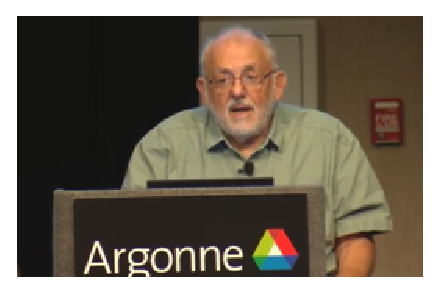
\includegraphics[width=0.9\linewidth]{Moler}
    \caption*{\index{Moler, Cleve}\textbf{Cleve Barry Moler}, (1939) 
              mathématicien et informaticien américain. Il est l'initiateur 
              du développement de MATLAB}
\end{marginfigure}
%-------------------------------------------------------------------------------
Les utilisateurs de MATLAB (environ 4 millions) sont de milieux très différents 
tels que l’ingénierie, les sciences et l’économie, dans un contexte aussi 
bien industriel que pour la recherche.
MATLAB peut s'utiliser seul ou bien avec des toolboxes (« boîte à outils »).
Le langage MATLAB est conçu par Cleve Moler à la fin des années 1970 à partir 
de deux bibliothèques écrites en Fortran : LINPACK et EISPACK4.
Alors professeur de mathématiques à l'université du Nouveau-Mexique, 
il souhaite permettre à ses étudiants d'utiliser ces deux bibliothèques sans 
connaître le Fortran. 
%\newpage
%%%%%%%%%%%%%%%%%%%%%%%%%%%%%%%%%%%%%%%%%%%%%%%%%%%%%%%%%%%%%%%%%%%%%%%%%%%%%%%%
%%%%%%%%%%%%%%%%%%%%%%%%%%%%%%%%%%%%%%%%%%%%%%%%%%%%%%%%%%%%%%%%%%%%%%%%%%%%%%%%
%%%%%%%%%%%%%%%%%%%%%%%%%%%%%%%%%%%%%%%%%%%%%%%%%%%%%%%%%%%%%%%%%%%%%%%%%%%%%%%%
\section{Présentation de l'environnemental MATLAB}
%%%%%%%%%%%%%%%%%%%%%%%%%%%%%%%%%%%%%%%%%%%%%%%%%%%%%%%%%%%%%%%%%%%%%%%%%%%%%%%%
%%%%%%%%%%%%%%%%%%%%%%%%%%%%%%%%%%%%%%%%%%%%%%%%%%%%%%%%%%%%%%%%%%%%%%%%%%%%%%%%
%%%%%%%%%%%%%%%%%%%%%%%%%%%%%%%%%%%%%%%%%%%%%%%%%%%%%%%%%%%%%%%%%%%%%%%%%%%%%%%%
La figure~\ref{fig-envMATLAB} illustre l'interface générale de MATLAB. 
Par défaut, on retrouve quatre fenêtres :
%-------------------------------------------------------------------------------
\begin{enumerate}
    \item \emph{Current Folder}
    \item \emph{Editor}
    \item \emph{Workspace}
    \item \emph{Command Window}
\end{enumerate}
%-------------------------------------------------------------------------------
%-------------------------------------------------------------------------------
\begin{figure}[!h]
    \centering
    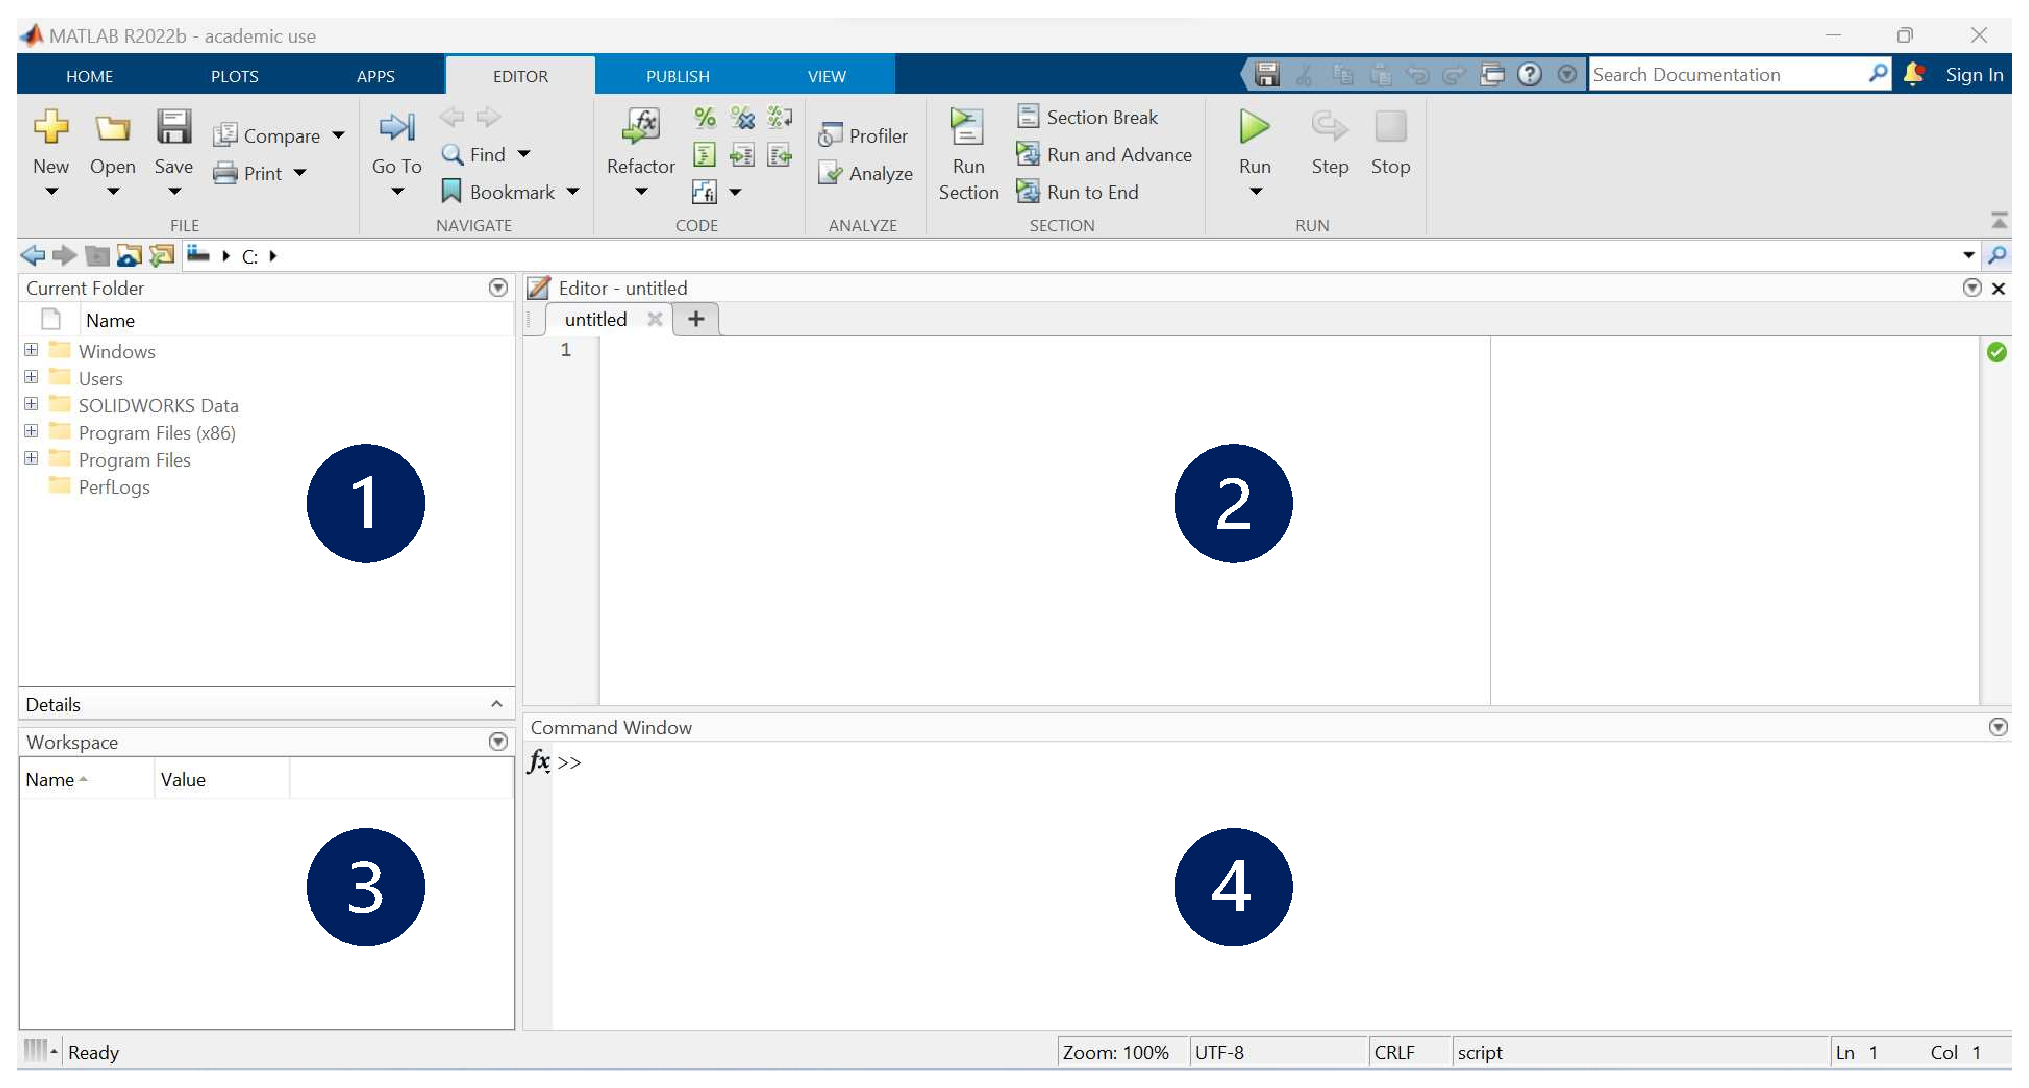
\includegraphics[width=0.9\linewidth]{fenetre_matlab-annexe_matlab.eps}
    \caption{Environnement de travail du logiciel MATLAB \label{fig-envMATLAB}}    
\end{figure}
%-------------------------------------------------------------------------------
\clearpage
%-------------------------------------------------------------------------------
\begin{marginfigure}
    \centering
    \includegraphics[width=0.9\linewidth]{current_folder-annexe_matlab.eps}
    \caption{Exemple de \emph{Current folder}\label{fig-CF}}    
\end{marginfigure}
%-------------------------------------------------------------------------------
\paragraph{\emph{Current Folder (1)}: } est le répertoire courant où sont 
enregistrés les fichiers. 

Exemple de fichiers 
\texttt{script\_exemple1.m} enregistré dans votre dossier de travail.

\paragraph{L'éditeur MATLAB (2): } est l'interface qui permet d'écrire
un ensemble d'instructions ou script. Il permet également de définir 
des fonctions. Il peut être lancé en tapant "edit NomDeFichier" dans le 
\emph{Command Window} ou en cliquant sur \verb?Home>>New Script?.
Un programme MATLAB (ou 'm-file' en anglais) est donc simplement
une suite d'instructions matlab écrites dans un éditeur de texte et 
sauvegardée dans un fichier d'extension \texttt{.m}.
%-------------------------------------------------------------------------------
\begin{figure}[!h]
    \centering
    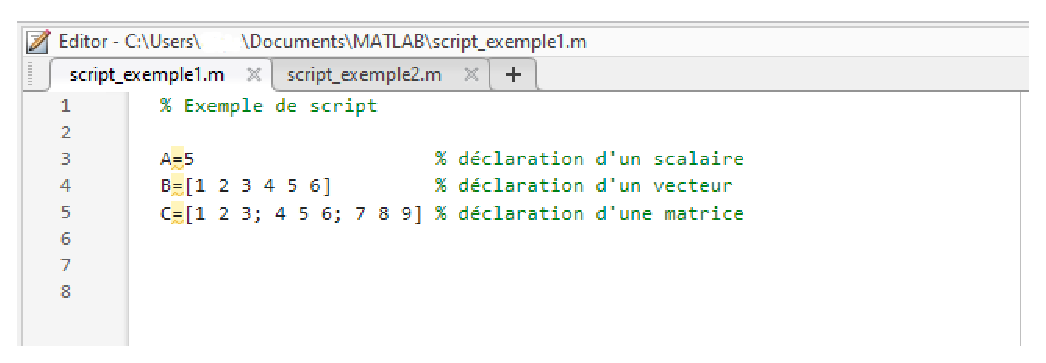
\includegraphics[width=\linewidth]{editor-annexe_matlab.eps}
\end{figure}
%-------------------------------------------------------------------------------
%-------------------------------------------------------------------------------
\begin{marginfigure}
    \centering
    \includegraphics[width=0.9\linewidth]{workspace-annexe_matlab.eps}
    \caption{Exemple de \emph{Workspace}\label{fig-Workspace}}    
\end{marginfigure}
%-------------------------------------------------------------------------------
\paragraph*{\emph{Workspace} (3): } permet de visualiser les variables mises 
en mémoire. On y retrouve leur nom, leur dimensions ainsi que le type 
de variable. MATLAB étant basé sur les matrices, toutes les
variables sont constituées de plusieurs dimensions.

\paragraph*{\emph{Command Window (4)}: } traite des instructions
données. Les résultats s'afficheront dès le retour de ligne. Le prompte 
commence toujours par \texttt{>}\,\texttt{>}. Si l'instruction ne 
comporte pas d'affectation, une variable \texttt{ans} est créée.
Le " ;" : Le point-virgule à la fin d'une ligne signale à MATLAB de ne pas
retourner le résultat de l'opération à l'écran.
%-------------------------------------------------------------------------------
\begin{marginfigure}
    \centering
    \includegraphics[width=0.9\linewidth]{command_window-annexe_matlab.eps}
    \caption{Exemple de \emph{Current Window}\label{fig-CW}}    
\end{marginfigure}
%-------------------------------------------------------------------------------
\clearpage
\restoregeometry
\captionsetup{width=0.9\linewidth}
%%%%%%%%%%%%%%%%%%%%%%%%%%%%%%%%%%%%%%%%%%%%%%%%%%%%%%%%%%%%%%%%%%%%%%%%%%%%%%%%
%%%%%%%%%%%%%%%%%%%%%%%%%%%%%%%%%%%%%%%%%%%%%%%%%%%%%%%%%%%%%%%%%%%%%%%%%%%%%%%%
%%%%%%%%%%%%%%%%%%%%%%%%%%%%%%%%%%%%%%%%%%%%%%%%%%%%%%%%%%%%%%%%%%%%%%%%%%%%%%%%
\section{Génération de signaux usuels}
%%%%%%%%%%%%%%%%%%%%%%%%%%%%%%%%%%%%%%%%%%%%%%%%%%%%%%%%%%%%%%%%%%%%%%%%%%%%%%%%
%%%%%%%%%%%%%%%%%%%%%%%%%%%%%%%%%%%%%%%%%%%%%%%%%%%%%%%%%%%%%%%%%%%%%%%%%%%%%%%%
%%%%%%%%%%%%%%%%%%%%%%%%%%%%%%%%%%%%%%%%%%%%%%%%%%%%%%%%%%%%%%%%%%%%%%%%%%%%%%%%
Dans un premier temps et afin de se familiariser avec MATLAB, nous 
allons d'abord construire les signaux en entrée $e(t)$, 
ainsi que la variable temporelle $t$.
Avant de commencer, éxécutez ces deux premières commandes qui permettent de 
nettoyer la fenêtre de commande et d'effacer toutes les variables 
enregistrées en mémoire.
\begin{minted}[bgcolor=col1!10]{matlab}
clc;
clear;
\end{minted}
%%%%%%%%%%%%%%%%%%%%%%%%%%%%%%%%%%%%%%%%%%%%%%%%%%%%%%%%%%%%%%%%%%%%%%%%%%%%%%%%
%%%%%%%%%%%%%%%%%%%%%%%%%%%%%%%%%%%%%%%%%%%%%%%%%%%%%%%%%%%%%%%%%%%%%%%%%%%%%%%%
\subsection{Vecteur temps}
%%%%%%%%%%%%%%%%%%%%%%%%%%%%%%%%%%%%%%%%%%%%%%%%%%%%%%%%%%%%%%%%%%%%%%%%%%%%%%%%
%%%%%%%%%%%%%%%%%%%%%%%%%%%%%%%%%%%%%%%%%%%%%%%%%%%%%%%%%%%%%%%%%%%%%%%%%%%%%%%%
La durée de la simulation est modélisée par un vecteur dont les composantes 
correspondent aux différents instants pour lesquels la réponse va être 
simulée. Par exemple le vecteur \texttt{t=[0 1 2 3 4 5]} modélisant le temps est
composée de 6 valeurs comprises entre 0 et 5. 
C'est à dire que la sortie sera évaluée en $s(0),s(1),\ldots,s(5)$.

Nous allons nons donner un vecteur \texttt{t} dont les éléments sont 
compris dans l'intervalle $[0,10[$ par des incréments de $0.01$. 
On pourra vérifier la taille de \texttt{t} à l'aide de la 
fonction \texttt{size}. On se donne également des variables \texttt{t\_start}, 
\texttt{t\_incr} et \texttt{t\_finish} qui permet de définir le vecteur 
\texttt{t} par la syntaxe suivante :
\begin{minted}[bgcolor=col1!10]{matlab}
>> t_start=0;
>> t_incr=0.01;
>> t_finish=10.0;
>> t=t_start:t_incr:t_finish;
>> size(t)
\end{minted}

\begin{minted}[bgcolor=col4!10]{text}
ans =

           1        1001
\end{minted}
\texttt{t} est donc un vecteur de 1001 composantes.
%%%%%%%%%%%%%%%%%%%%%%%%%%%%%%%%%%%%%%%%%%%%%%%%%%%%%%%%%%%%%%%%%%%%%%%%%%%%%%%%
%%%%%%%%%%%%%%%%%%%%%%%%%%%%%%%%%%%%%%%%%%%%%%%%%%%%%%%%%%%%%%%%%%%%%%%%%%%%%%%%
\subsection{Génération d'un échelon}
%%%%%%%%%%%%%%%%%%%%%%%%%%%%%%%%%%%%%%%%%%%%%%%%%%%%%%%%%%%%%%%%%%%%%%%%%%%%%%%%
%%%%%%%%%%%%%%%%%%%%%%%%%%%%%%%%%%%%%%%%%%%%%%%%%%%%%%%%%%%%%%%%%%%%%%%%%%%%%%%%
L'échelon d'amplitude $A$ définie par:
\[
    u(t)=\begin{cases}
        1 \qquad \textrm{si} \quad t\geq 0 \\
        0 \qquad \textrm{si} \quad t<0
         \end{cases}
\]
Nous pouvons utiliser la fonctiones \texttt{ones} qui retourne un vecteur 
de un de taille quelconque :  
%-------------------------------------------------------------------------------
\begin{minted}[bgcolor=col1!10]{matlab}
>> N = 1001;
>> e_echelon = ones (1,N);
>> size(e_echelon)
\end{minted}
%-------------------------------------------------------------------------------
%-------------------------------------------------------------------------------
\begin{minted}[bgcolor=col4!10]{text}
ans =

           1        1001
\end{minted}
%-------------------------------------------------------------------------------
Il est préférable de définir \texttt{u} à partir de la taille de \texttt{t} :
%-------------------------------------------------------------------------------
\begin{minted}[bgcolor=col1!10]{matlab}
>> e_echelon = A * ones (size(t));
\end{minted}
%-------------------------------------------------------------------------------
%%%%%%%%%%%%%%%%%%%%%%%%%%%%%%%%%%%%%%%%%%%%%%%%%%%%%%%%%%%%%%%%%%%%%%%%%%%%%%%%
%%%%%%%%%%%%%%%%%%%%%%%%%%%%%%%%%%%%%%%%%%%%%%%%%%%%%%%%%%%%%%%%%%%%%%%%%%%%%%%%
\subsection{Génération d'une rampe}
%%%%%%%%%%%%%%%%%%%%%%%%%%%%%%%%%%%%%%%%%%%%%%%%%%%%%%%%%%%%%%%%%%%%%%%%%%%%%%%%
%%%%%%%%%%%%%%%%%%%%%%%%%%%%%%%%%%%%%%%%%%%%%%%%%%%%%%%%%%%%%%%%%%%%%%%%%%%%%%%%
L'intégrale de la fonction $u(t)$ par rapport au temps est la fonction rampe 
$r(t)$. Ce nouveau signal est défini par:
\[
    r(t)=\begin{cases}
        t \qquad \textrm{si} \quad  t\geq 0
        0 \qquad \textrm{si} \quad  t<0
         \end{cases}
\]
La rampe $r(t)$ peut être générée en utilisant la commande MATLAB suivante:
%-------------------------------------------------------------------------------
\begin{minted}[bgcolor=col1!10]{matlab}
>> e_rampe = t;
>> size(e_rampe)
\end{minted}
%-------------------------------------------------------------------------------
%-------------------------------------------------------------------------------
\begin{minted}[bgcolor=col4!10]{text}
ans =

           1        1001
\end{minted}
%-------------------------------------------------------------------------------
%%%%%%%%%%%%%%%%%%%%%%%%%%%%%%%%%%%%%%%%%%%%%%%%%%%%%%%%%%%%%%%%%%%%%%%%%%%%%%%%
%%%%%%%%%%%%%%%%%%%%%%%%%%%%%%%%%%%%%%%%%%%%%%%%%%%%%%%%%%%%%%%%%%%%%%%%%%%%%%%%
\subsection{Génération d'une impulsion de Dirac}
%%%%%%%%%%%%%%%%%%%%%%%%%%%%%%%%%%%%%%%%%%%%%%%%%%%%%%%%%%%%%%%%%%%%%%%%%%%%%%%%
%%%%%%%%%%%%%%%%%%%%%%%%%%%%%%%%%%%%%%%%%%%%%%%%%%%%%%%%%%%%%%%%%%%%%%%%%%%%%%%%
Dans le cas de l'impulsion de Dirac, nous allons approché le signal d'entrée par 
la fonction $\delta_a$ où $a$ est l'intervalle entre deux valeurs de \texttt{t}. 
Cette approximation est nécessaire dans un contexte numérique
(échantillonner) ou la distribution de Dirac est mal définie. 
%-------------------------------------------------------------------------------
\begin{figure}[!h]
    \centering
    \tikzsetnextfilename{dirac_reel-chap_slci-ext}
    \input{tikz/dirac_reel-chap_slci.tex}
    \caption{Représentation de l'impulsion de Dirac approchée. 
             Celle-ci tend vers l'impulsion de Dirac pour $a\to0$. 
             On remarquera que l'aire du rectangle est toujours égale à 1.
             \label{fig-dirac2}}
\end{figure}
%-------------------------------------------------------------------------------
%-------------------------------------------------------------------------------
\begin{minted}[bgcolor=col1!10]{matlab}
>> e_dirac=zeros(size(t));
>> e_dirac(1)=1/t_incr;
>> size(e_dirac)
\end{minted}
%-------------------------------------------------------------------------------
%%%%%%%%%%%%%%%%%%%%%%%%%%%%%%%%%%%%%%%%%%%%%%%%%%%%%%%%%%%%%%%%%%%%%%%%%%%%%%%%
%%%%%%%%%%%%%%%%%%%%%%%%%%%%%%%%%%%%%%%%%%%%%%%%%%%%%%%%%%%%%%%%%%%%%%%%%%%%%%%%
%%%%%%%%%%%%%%%%%%%%%%%%%%%%%%%%%%%%%%%%%%%%%%%%%%%%%%%%%%%%%%%%%%%%%%%%%%%%%%%%
\section{Systèmes linéaires, continus et invariants}
%%%%%%%%%%%%%%%%%%%%%%%%%%%%%%%%%%%%%%%%%%%%%%%%%%%%%%%%%%%%%%%%%%%%%%%%%%%%%%%%
%%%%%%%%%%%%%%%%%%%%%%%%%%%%%%%%%%%%%%%%%%%%%%%%%%%%%%%%%%%%%%%%%%%%%%%%%%%%%%%%
%%%%%%%%%%%%%%%%%%%%%%%%%%%%%%%%%%%%%%%%%%%%%%%%%%%%%%%%%%%%%%%%%%%%%%%%%%%%%%%%
%%%%%%%%%%%%%%%%%%%%%%%%%%%%%%%%%%%%%%%%%%%%%%%%%%%%%%%%%%%%%%%%%%%%%%%%%%%%%%%%
%%%%%%%%%%%%%%%%%%%%%%%%%%%%%%%%%%%%%%%%%%%%%%%%%%%%%%%%%%%%%%%%%%%%%%%%%%%%%%%%
\subsection{Représentation des polynômes avec MATLAB}
%%%%%%%%%%%%%%%%%%%%%%%%%%%%%%%%%%%%%%%%%%%%%%%%%%%%%%%%%%%%%%%%%%%%%%%%%%%%%%%%
%%%%%%%%%%%%%%%%%%%%%%%%%%%%%%%%%%%%%%%%%%%%%%%%%%%%%%%%%%%%%%%%%%%%%%%%%%%%%%%%
Les polynômes sont représentés sous MATLAB par des vecteurs ordonnés selon 
les puissances décroissantes.
Par exemple, le polynôme $P(x)=x^2+3x+2$ est représenté par le vecteur :
%-------------------------------------------------------------------------------
\begin{minted}[bgcolor=col1!10]{matlab}
>> p = [ 1  3  2 ]
\end{minted}
%-------------------------------------------------------------------------------
ou encore le polynôme $Q(x)=4x^5−3x^2+2x+33$ est représenté par le vecteur :
%-------------------------------------------------------------------------------
\begin{minted}[bgcolor=col1!10]{matlab}
>> q = [ 4 0 0 -3 2 33 ]
\end{minted}
%-------------------------------------------------------------------------------
Pour évaluer le polynôme en une valeur spécifique, on utilisera la fonction 
\texttt{polyval}. Par exemple, pour évaluer le polynôme $P(x)$ précédent en $x=2$,
on écrira l'instruction suivante :
%-------------------------------------------------------------------------------
\begin{minted}[bgcolor=col1!10]{matlab}
>> polyval(q,2)
\end{minted}
%-------------------------------------------------------------------------------
%-------------------------------------------------------------------------------
\begin{minted}[bgcolor=col4!10]{text}
ans =

   153
\end{minted}
%-------------------------------------------------------------------------------
Pour déterminer les racines d'un polynôme, on utilisera la fonction \texttt{roots}.
Par exemple, les racines du polynôme $P(x)=2x^2+3x+2$ sont données par l'instruction
suivante :
%-------------------------------------------------------------------------------
\begin{minted}[bgcolor=col1!10]{matlab}
>> p = [ 1  3  2 ];
>> roots(p)
\end{minted}
%-------------------------------------------------------------------------------
%-------------------------------------------------------------------------------
\begin{minted}[bgcolor=col4!10]{text}
ans =

    -2
    -1
\end{minted}
%-------------------------------------------------------------------------------
-2 et -1 étants les racines de $P(x)$.

Il est également possible de définir un polynôme à partir de ces racines avec 
la fonction \texttt{poly}. Ainsi l'instruction suivante donne le polynôme $P(x)$:
%-------------------------------------------------------------------------------
\begin{minted}[bgcolor=col1!10]{matlab}
>> p = [ 1  3  2 ];
>> poly(p)
\end{minted}
%-------------------------------------------------------------------------------
%-------------------------------------------------------------------------------
\begin{minted}[bgcolor=col4!10]{text}
ans =

     1     3     2
\end{minted}
%-------------------------------------------------------------------------------
\clearpage
\input{re/newgeometry}
\captionsetup{width=0.9\linewidth}
%%%%%%%%%%%%%%%%%%%%%%%%%%%%%%%%%%%%%%%%%%%%%%%%%%%%%%%%%%%%%%%%%%%%%%%%%%%%%%%%
%%%%%%%%%%%%%%%%%%%%%%%%%%%%%%%%%%%%%%%%%%%%%%%%%%%%%%%%%%%%%%%%%%%%%%%%%%%%%%%%
\subsection{Représentation d'une fonction de transfert}
%%%%%%%%%%%%%%%%%%%%%%%%%%%%%%%%%%%%%%%%%%%%%%%%%%%%%%%%%%%%%%%%%%%%%%%%%%%%%%%%
%%%%%%%%%%%%%%%%%%%%%%%%%%%%%%%%%%%%%%%%%%%%%%%%%%%%%%%%%%%%%%%%%%%%%%%%%%%%%%%%
Une fonction de transfert est un fraction rationnelle 
(i.e un rapport de polynôme). C'est à l'aide de la fonction MATLAB \texttt{tf()}
que nous pourrons définir une fonction de transfert. Par exemple, si 
l'on souhaite représenter la fonction de transfert du premier ordre $H(s)$ :
\[
    H(s) = \dfrac{1}{s+1}
\]
C'est à dire un polynôme de degré zéro au numérateur et un polynôme de 
degré 1 au dénominateur\footnote{Nous utiliserons l'indéterminée du polynôme $s$ 
en lieu et place de $p$ pour suivre la notation employée par MATLAB}, on écrira
l'instruction suivante :
%-------------------------------------------------------------------------------
\begin{minted}[bgcolor=col1!10]{matlab}
>> H=tf(1,[1 1]) 
\end{minted}
%-------------------------------------------------------------------------------
%-------------------------------------------------------------------------------
\begin{minted}[bgcolor=col4!10]{text}
H =
 
    1
  -----
  s + 1
 
Continuous-time transfer function.
\end{minted}
%-------------------------------------------------------------------------------
où le premier argument correspond aux coefficients du polynôme au numérateur 
et le second sont les coefficients du polynôme au dénominateur. 
%-------------------------------------------------------------------------------
\begin{marginfigure}
    \centering
    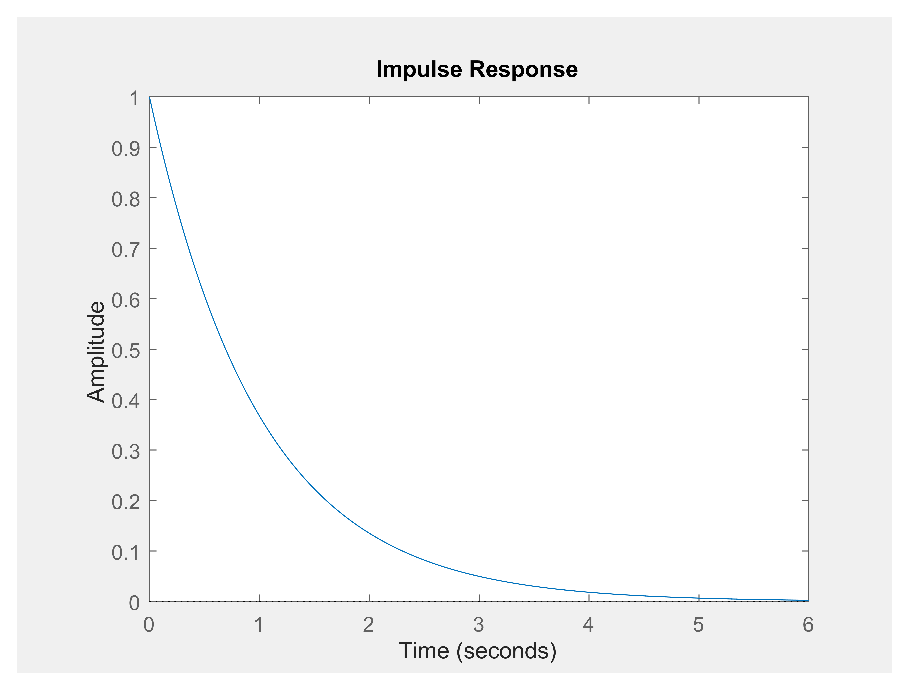
\includegraphics[width=0.9\linewidth]{impulse_1er-annexe_matlab.eps}
    \caption{Réponse impulsionnelle obtenue par la fonction \texttt{impulse} de MATLAB}
\end{marginfigure}
%-------------------------------------------------------------------------------
%-------------------------------------------------------------------------------
\begin{marginfigure}
    \centering
    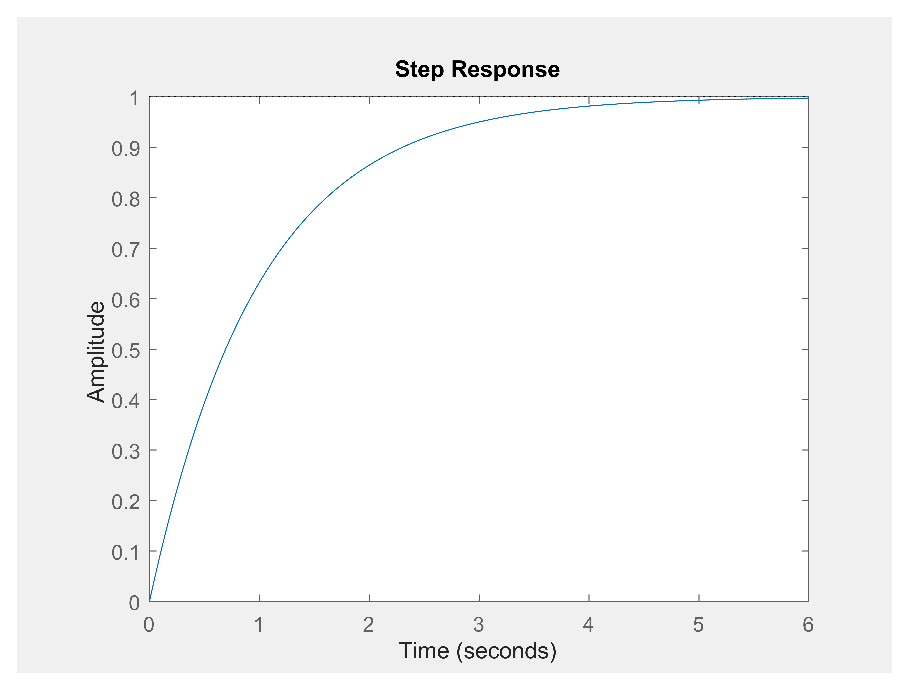
\includegraphics[width=0.9\linewidth]{step_1er-annexe_matlab.eps}
    \caption{Réponse impulsionnelle obtenue par la fonction \texttt{step} de MATLAB}
\end{marginfigure}
%-------------------------------------------------------------------------------
%%%%%%%%%%%%%%%%%%%%%%%%%%%%%%%%%%%%%%%%%%%%%%%%%%%%%%%%%%%%%%%%%%%%%%%%%%%%%%%%
%%%%%%%%%%%%%%%%%%%%%%%%%%%%%%%%%%%%%%%%%%%%%%%%%%%%%%%%%%%%%%%%%%%%%%%%%%%%%%%%
\subsection{Réponses temporelles}
%%%%%%%%%%%%%%%%%%%%%%%%%%%%%%%%%%%%%%%%%%%%%%%%%%%%%%%%%%%%%%%%%%%%%%%%%%%%%%%%
%%%%%%%%%%%%%%%%%%%%%%%%%%%%%%%%%%%%%%%%%%%%%%%%%%%%%%%%%%%%%%%%%%%%%%%%%%%%%%%%
Pour rappel, les réponses temporelles consistent à déterminer les sorties 
d'un système pour les différentes sollicitations usuelles, notamment :
\begin{itemize}
    \item La réponse impulsionnelle correspond à la réponse à une impulsion de Dirac
    \item La réponse indicielle correspond à la réponse à un échelon unitaire
    \item La réponse à une rampe correspond à la réponse à un signal rampe
\end{itemize}
%%%%%%%%%%%%%%%%%%%%%%%%%%%%%%%%%%%%%%%%%%%%%%%%%%%%%%%%%%%%%%%%%%%%%%%%%%%%%%%%
\subsubsection{Fonctions prédéfinies}
%%%%%%%%%%%%%%%%%%%%%%%%%%%%%%%%%%%%%%%%%%%%%%%%%%%%%%%%%%%%%%%%%%%%%%%%%%%%%%%%
Il existe des fonctions prédéfinies pour le calcul et le tracer des 
réponses impulsionnelles et indicielles. Respectivement \texttt{impulse} et \texttt{step} :
%-------------------------------------------------------------------------------
\begin{minted}[bgcolor=col1!10]{matlab}
>> impulse(H);
>> step(H);
\end{minted}
%-------------------------------------------------------------------------------
Sans affectation, ces fonctions tracent les réponses temporelles du système pour 
un interval de temps et une durée déterminés par la fonction \texttt{impulse} 
elle-même.
Il est également possible de récupérer la réponse temporelle sous forme 
de vecteurs colonnes en sortie de ces fonctions. D'autres arguments permettent 
de définir spécifiquement le temps de la simulation.
On se retournera vers le manuel d'utilisation des 
fonctions \href{https://fr.mathworks.com/help/control/ref/dynamicsystem.impulse.html}{impulse} 
et \href{https://fr.mathworks.com/help/control/ref/dynamicsystem.step.html}{step}~\cite{impulse,step}
%%%%%%%%%%%%%%%%%%%%%%%%%%%%%%%%%%%%%%%%%%%%%%%%%%%%%%%%%%%%%%%%%%%%%%%%%%%%%%%%
\subsubsection{Calcul de la réponse à une entrée quelconque}
%%%%%%%%%%%%%%%%%%%%%%%%%%%%%%%%%%%%%%%%%%%%%%%%%%%%%%%%%%%%%%%%%%%%%%%%%%%%%%%%
La fonction \texttt{lsim} permet de simuler et de tracer 
la réponse temporelle d'un système pour une entrée quelconque et un vecteur
temps donné. 
Par exemple, on souhaite déterminer la réponse temporelle 
d'un système \texttt{H} pour une sollicitation $e(t)$ telle que :
\[
    e(t)= \begin{cases}
        1\quad \textrm{pour}\quad t<\tau \\
        0\quad \textrm{pour}\quad t>\tau 
          \end{cases}
\]
%-------------------------------------------------------------------------------
\begin{marginfigure}
    \centering
    \tikzsetnextfilename{entreequelconque-annexe_matlab-ext}
    \begin{tikzpicture}
    \begin{axis}
    [   ticks=none,
        axis line style = thick,
        height=5cm,
        width=5cm,
        axis x line=center,
        axis y line=center,
        xmin=-2,
        xmax=4,
        ymin=-1.5,
        ymax=3.0,
        xlabel={$t$},
        ylabel={$e(t)$},
        xlabel style={below right},
        ylabel style={above left}
    ]
    \addplot [signalb,domain=-2:0] {0};
    \addplot [signalb,domain=0:2 ] {2};
    \addplot [signalb,domain=2:5 ] {0};
    \draw[dotted,very thick,col1] (axis cs:0,0) -- (axis cs:0,2);
    \draw[dotted,very thick,col1] (axis cs:2,2) -- (axis cs:2,0);
    \node[col1] at (axis cs:2,-0.5) {$\tau$};
    \node[col1] at (axis cs:-0.5,2) {$1$};
    \end{axis}
\end{tikzpicture}

    \caption{Sollicitation $e(t)$ en entrée de \texttt{H}}
\end{marginfigure}
%-------------------------------------------------------------------------------
Les instructions suivantes permettent le tracer de cette réponse temporelle
à l'aide de la fonction \texttt{lsim}.
%-------------------------------------------------------------------------------
\begin{minted}[bgcolor=col1!10]{matlab}
% nombre de points simulé 
nsamp=256
% t0 = 0 
% tf = 10
% nombre de points 
t=linspace(0,10,nsamp);
% e(t) = 1 pour         0 < t < nsamp/2
% e(t) = 0 pour nsamp/2+1 < t < nsamp
e=[ones(1,nsamp/2) zeros(1,nsamp/2)] 
% fonction de transfert
H=tf(1,[1 1])
%réponse de H par e
s=lsim(H,e,t) 
plot(t,s)
\end{minted}
%-------------------------------------------------------------------------------
Nous nous reporterons à la documentation officielle pour obtenir davantage de
détails sur les arguments et les retours de cette fonction 
\href{https://fr.mathworks.com/help/control/ref/dynamicsystem.lsim.html}{\texttt{lsim}}~\cite{lsim}.
%-------------------------------------------------------------------------------
\begin{marginfigure}
    \centering
    \includegraphics[width=0.9\linewidth]{reponse_quelconque-annexe_matlab.eps}
    \caption{Tracé de la réponse à la sollicitation $e(t)$ quelconque}
\end{marginfigure}
%-------------------------------------------------------------------------------
\clearpage
\restoregeometry
\captionsetup{width=0.9\linewidth}
%%%%%%%%%%%%%%%%%%%%%%%%%%%%%%%%%%%%%%%%%%%%%%%%%%%%%%%%%%%%%%%%%%%%%%%%%%%%%%%%
\section{Exemple d'application}
%%%%%%%%%%%%%%%%%%%%%%%%%%%%%%%%%%%%%%%%%%%%%%%%%%%%%%%%%%%%%%%%%%%%%%%%%%%%%%%%
Soit la fonction de transfert d'un système de premier ordre :
\[
    H(p)=\frac{1}{1+\tau p}
\]
On souhaiter étudier les réponses indicielles pour différentes valeurs
de $\tau=\{5,10,20\}$. On donne le script complet pour l'étude 
\begin{minted}[bgcolor=col1!10]{matlab}
%gain
K=1
%temps caractéristiques
tau=[5 10 20];
%vecteur temps
t=linspace(0,80,256)
hold on
%boucle sur toutes les valeurs de tau
for k=1:3
    H=tf(K,[tau(k) 1])
    step(H,t)
end
\end{minted}
%-------------------------------------------------------------------------------
\begin{figure}[!h]
    \centering
    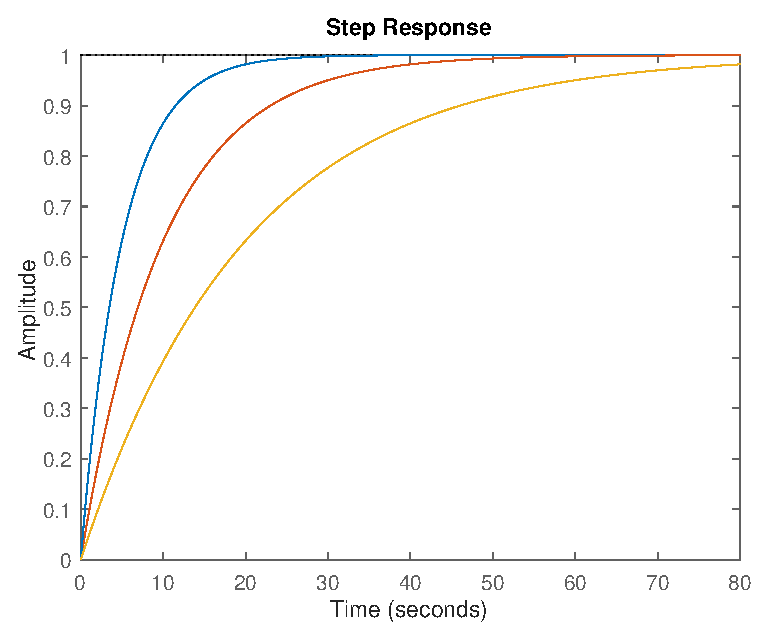
\includegraphics[width=0.9\linewidth]{exemple-annexe_matlab.eps}
    \caption{Simulation avec MATLAB de le réponse indicielle pour trois 
             valeurs de $\tau$.}
\end{figure}
%-------------------------------------------------------------------------------

%annexe_matlab.tex
